\documentclass[11pt]{article}

\usepackage[utf8]{inputenc}
\usepackage[T1]{fontenc}
\usepackage{lmodern}
\usepackage{CJKutf8}
\usepackage{amsmath,amssymb}
\usepackage{booktabs}
\usepackage{graphicx}
\usepackage{microtype}
\usepackage[round,authoryear]{natbib}
\usepackage{url}
\usepackage[hidelinks]{hyperref}
\usepackage[margin=1in]{geometry}
\usepackage{caption}
\usepackage{placeins}

\captionsetup{font=small,labelfont=bf}
\setlength{\parindent}{1.3em}
\setlength{\parskip}{0pt}
\setlength{\emergencystretch}{2em}

\title{Capacity-Constrained Uplift Modelling on CRITEO-UPLIFTv2:\\
Held-Out Policy Evaluation}
\author{Yi Zhao}
\date{August 2026}

\begin{document}
\maketitle

\begin{abstract}
Targeting systems often rank users by their predicted outcome under treatment, although the decision objective is the incremental effect of treatment. Whether a conditional treatment effect score improves a capacity-constrained allocation is an empirical question. This study compares expected uniform random allocation, treated-response ranking, a T-learner, and a three-fold cross-fitted doubly robust learner on the corrected CRITEO-UPLIFTv2 benchmark. The analysis uses 13,979,592 records from randomized advertising experiments, a fixed 60/20/20 split, and conversion as the primary outcome. Fitted models and score definitions were frozen before the evaluation routine loaded test outcome columns or joined them to predictions. Policies were then evaluated at capacities of 5\%, 10\%, 20\%, 50\%, and 100\% with held-out augmented inverse-probability-weighted value estimates. Pointwise uncertainty comes from 1,000 paired row-bootstrap replicates conditional on the fitted models. The complete-source conversion average treatment effect was 0.1152 percentage points (95\% confidence interval 0.1085 to 0.1219). At 10\% capacity, treated-response ranking exceeded expected random allocation by 77.3 incremental conversions per 100,000 test users (pointwise 95\% interval 65.1 to 90.0). Its estimated value also exceeded the T-learner by 9.0 (1.8 to 15.3) and the doubly robust learner by 29.7 (21.8 to 37.5) per 100,000. Treated-response ranking had the highest estimated conversion value at every constrained capacity; all policies were identical at 100\% by construction. These results are an offline benchmark comparison, not evidence of realized campaign impact or monetary return.
\end{abstract}

\noindent\textbf{Keywords:} uplift modelling; heterogeneous treatment effects; policy evaluation; capacity constraints; doubly robust learning; randomized experiments

\begin{CJK*}{UTF8}{gbsn}
\section*{摘要}
投放系统常按照用户接受处理后的预测结果排序，但实际决策目标是处理带来的增量效果。本文使用修正后的 CRITEO-UPLIFTv2 公开数据，比较均匀随机分配、处理条件下的预测反应分数、T-learner 与三折交叉拟合的 doubly robust learner。数据包含 13,979,592 条随机广告实验记录，主要结局为转化，并采用固定的训练、验证和测试划分。在评估程序载入测试结局列或将其与预测结果合并之前，拟合模型与评分规则均已固定。本文在 5\%、10\%、20\%、50\% 与 100\% 容量下，使用测试集的 augmented inverse-probability-weighted policy value 进行评估；不确定性通过 1,000 次配对 bootstrap 估计，每次均对测试行重抽样；所得区间是在模型保持固定条件下计算的逐点 95\% 百分位区间。全部数据的转化平均处理效应为 0.1152 个百分点。容量为 10\% 时，处理条件下的预测反应排序相较随机分配，每十万名测试用户的预计增量转化高 77.3 次，区间为 65.1 至 90.0；其估计值也比 T-learner 高 9.0 次，并比 doubly robust learner 高 29.7 次。处理条件下的预测反应排序在所有受限容量下均有最高的转化 policy value 估计值，而 100\% 容量下各策略依定义相同。结果只描述公开基准数据中的离线政策评估，不代表已经实现的广告成效或货币回报。

\noindent\textbf{关键词：} uplift modelling；异质处理效应；政策评估；容量限制；双重稳健学习；随机实验
\end{CJK*}

\section{Introduction}

A conversion model answers which users are likely to convert after receiving an advertisement. A targeting policy needs a different quantity: which users are more likely to convert because they receive it. The two rankings can disagree because a user with high baseline demand may have a high treated outcome probability but little incremental response. Uplift modelling and heterogeneous treatment effect estimation address this distinction by estimating differences between potential outcomes \citep{kunzel2019metalearners,diemert2021benchmark}.

The distinction matters when only a fraction of eligible users can be treated. A score is useful in that setting only if the induced allocation has high incremental value at the relevant capacity. Predictive loss, conditional effect error, and ranking diagnostics describe parts of this problem, but none by itself supplies a held-out estimate of the resulting policy value. Policy learning work instead treats allocation as a statistical decision problem and evaluates a policy by the outcomes it would change \citep{kitagawa2018treatment,athey2021policy}. Doubly robust estimators combine outcome regression with inverse probability weighting and are widely used for offline policy evaluation \citep{dudik2011dr}.

This paper studies a concrete question on the corrected CRITEO-UPLIFTv2 dataset: under fixed treatment capacity, do treatment effect rankings yield higher held-out estimated incremental conversions than a treated-response ranking? Four pre-specified rules are compared: expected exact-size random allocation, ranking by predicted conversion under treatment, ranking by a T-learner effect estimate, and ranking by a cross-fitted doubly robust effect estimate. The primary endpoint is conversion. Visit is evaluated as a secondary outcome for the same conversion-based policies.

The study does not introduce a new learner. It provides a reproducible case study in which the data split, model selection, ranking-score definitions, capacities, tie-breaking rule, estimands, and contrasts were fixed before the evaluation routine loaded test outcome columns or joined them to predictions. Three quantities remain separate throughout the analysis: the complete-source difference-in-means average treatment effect, held-out augmented inverse-probability-weighted (AIPW) policy value, and a centered fixed-propensity inverse-probability-weighted (IPW) Qini diagnostic. This separation prevents a ranking metric or an in-sample effect estimate from being presented as policy performance.

In this comparison, the treatment-effect scores did not rank best: treated-response ranking had the highest estimated conversion policy value at capacities from 5\% through 50\%. This result is specific to these learners, this release, and this evaluation design; it does not show that response models are generally preferable to treatment-effect models.

\section{Related work}

\subsection{Uplift and heterogeneous treatment effect estimation}

Meta-learners reduce conditional average treatment effect (CATE) estimation to supervised regression problems. The T-learner fits separate response surfaces by treatment arm and subtracts their predictions \citep{kunzel2019metalearners}. This flexibility can help when the two surfaces differ, but the subtraction carries estimation error from both models. Doubly robust CATE methods regress an orthogonal pseudo-outcome on covariates, combining response surfaces and treatment probabilities \citep{kennedy2023dr}. Cross-fitting reduces the dependence between each pseudo-outcome and the nuisance estimates used to construct it \citep{chernozhukov2018dml}.

The Criteo benchmark made large randomized advertising data available for uplift research \citep{diemert2018benchmark,diemert2021benchmark}. Work using uplift curves and learning-to-rank objectives has emphasized that a model may be judged by ordering quality rather than pointwise effect accuracy \citep{betlei2021uplift,devriendt2022rank}. This paper retains a centered Qini curve as a ranking diagnostic, but makes held-out policy value at specified capacities the decision-facing target.

\subsection{Policy choice and offline evaluation}

Empirical welfare maximization frames treatment assignment as direct optimization over a policy class \citep{kitagawa2018treatment}. Related work derives policy learners and regret guarantees from semiparametric scores, including settings with budget or structural constraints \citep{athey2021policy}. Doubly robust policy evaluation combines a response model with importance weighting so that errors in one nuisance component can be offset under suitable conditions \citep{dudik2011dr}. The present experiment is simpler because assignment probability is known and constant. Its policy class is a frozen set of score rankings with exact capacity cutoffs.

Outcome prediction remains a meaningful comparator. \citet{fernandezloria2022causal} show that causal classification can exhibit a bias-variance tradeoff: a biased outcome score may make better treatment decisions than an estimated effect score when the latter is noisy. Their analysis gives one reason a treated-response ranking can outperform a ranking based on estimated treatment effects in finite samples, but it does not predict when this will occur.

\section{Data and study design}

\subsection{Dataset and analysis population}

CRITEO-UPLIFTv2 contains observations collected from several randomized advertising trials. The corrected public artifact, labeled v2.1 by the publisher, removes a treatment-ratio leakage problem reported for the earlier release \citep{diemert2021benchmark}. The file used here contains 13,979,592 rows, twelve anonymous pre-treatment features, randomized treatment assignment, conversion, visit, and exposure. The source describes four features as continuous and eight as categorical. Treatment probability is 0.85 \citep{criteoDataset,diemert2021benchmark}.

Treatment denotes randomized assignment. Exposure is realized after assignment, so it is excluded from all features, estimands, scores, and policies. The analysis therefore estimates intention-to-treat effects, not effects among exposed users. The release is anonymized and was sampled by its publisher for benchmark use. Results target the released-data distribution, not population-weighted advertising traffic.

The raw gzip file has the following SHA-256 digest:
\begin{center}
\texttt{\small 2716e1bf0fd157a93b5bf86924d90884}\\
\texttt{\small 19dfbac2022c6cd90030220634f616dc}.
\end{center}
Before fitting, the pipeline checked the ordered schema, row count, finite feature values, binary domains, the absence of exposure in controls, and the implication from conversion to visit. Repeated anonymous rows were retained because no documented user identifier is available.

\subsection{Fixed split and descriptive checks}

A zero-based source-order identifier was hashed with seed 20260803 into ten buckets. Six buckets formed the training set (8,386,222 rows), two formed validation (2,796,279), and two formed the held-out test set (2,797,091). The identifier was never used as a feature. Categorical levels were learned on training covariates and then reused without modification.

Randomization diagnostics used training and validation rows only. Continuous features were summarized by pooled-standard-deviation standardized mean differences (SMDs). Each categorical feature was summarized by the largest absolute one-versus-rest SMD across its levels. A treatment classifier fitted on training covariates and scored on validation covariates supplied a joint descriptive check. Neither the 0.1 SMD reference line nor classifier area under the curve (AUC) was treated as a formal randomization test.

Table~\ref{tab:test-sample} describes the held-out test assignments and outcomes. These raw rates are descriptive. Policy comparisons use the estimators defined below.

\begin{table}[htbp]
\centering
\caption{Held-out test sample by randomized assignment. Rates are observed sample proportions.}
\label{tab:test-sample}
\resizebox{\textwidth}{!}{\begin{tabular}{@{}lrrrrr@{}}
\toprule
Assignment & Rows & Conversions & Conversion rate (\%) & Visits & Visit rate (\%) \\
\midrule
Control & 419,300 & 814 & 0.1941 & 16,110 & 3.8421 \\
Treated & 2,377,791 & 7,255 & 0.3051 & 115,108 & 4.8410 \\
\bottomrule
\end{tabular}
}
\end{table}

\section{Estimands and methods}

\subsection{Average treatment effects}

Let $T_i\in\{0,1\}$ denote randomized assignment and let $Y_i(t)$ be the potential outcome under assignment $t$. Conversion is the primary outcome and visit is secondary. The complete-source average treatment effect (ATE) is
\[
\tau_Y = \mathbb{E}\{Y_i(1)-Y_i(0)\}.
\]
It is estimated by the difference in assignment-group means,
\[
\widehat{\tau}_Y=\overline{Y}_1-\overline{Y}_0,
\qquad
\widehat{\operatorname{SE}}(\widehat{\tau}_Y)
=\sqrt{\frac{s_1^2}{n_1}+\frac{s_0^2}{n_0}},
\]
with a normal 95\% confidence interval. This complete-source descriptive estimand is reported separately from policy evaluation on the test split.

Identification of the ATE and policy values uses the publisher-reported randomized assignment with known $0<e_0=0.85<1$, consistency, and no interference across records. The normal ATE interval and paired row bootstrap further treat rows as exchangeable IID draws from the released-data distribution. User and campaign identifiers are unavailable, so repeated-user dependence, clustering, and cross-record interference cannot be checked.

\subsection{Capacity-constrained batch policies}

For an evaluation batch of $n$ users and capacity $q$, let $k=\lfloor qn\rfloor$. A deterministic hash
\[
U_i=H(20260803,\operatorname{row\_id}_i)
\]
breaks score ties. A score $s$ induces the batch policy $\Pi_{s,q}$ that treats the first $k$ users ordered by decreasing $s(X_i)$ and then increasing $U_i$. Its incremental outcome value per eligible test row is
\[
\Delta_{Y,n}(\Pi_{s,q})
=\mathbb{E}\left[
\frac{1}{n}\sum_{i=1}^{n}
\pi_{s,q,i}\{Y_i(1)-Y_i(0)\}
\right].
\]
Because membership depends on the other scores in the batch, this is an exact-size allocation rule rather than an independent threshold rule.

Five capacities were fixed: 5\%, 10\%, 20\%, 50\%, and 100\%. Capacity represents equal-cost treatment slots. The source contains neither treatment cost nor conversion value, so the analysis does not estimate profit, return on investment, or a monetary budget frontier.

\subsection{Scores and fitted models}

The random benchmark is the expected policy value of an exact-size allocation that samples $k$ users uniformly without replacement. Three fitted scores are compared with it:
\[
\begin{aligned}
s_{\mathrm{response}}(x) &= \widehat m_1^C(x),\\
s_{\mathrm{T}}(x) &= \widehat m_1^C(x)-\widehat m_0^C(x),\\
s_{\mathrm{DR}}(x) &= \widehat\tau_{\mathrm{DR}}(x),
\end{aligned}
\]
where $C$ denotes conversion. The first score is a treated-response prediction, not a propensity score.

LightGBM binary classifiers estimate the arm-specific conversion and visit response surfaces. The treatment probability is fixed at the design value $e_0=0.85$. No class weighting, outcome downsampling, probability calibration tournament, or hyperparameter sweep was used. Boosting rounds for each arm-specific model were selected by validation log-loss.

The DR-learner uses three-fold cross-fitting on the combined training and validation data. For development row $i$ in fold $f$, its conversion pseudo-outcome is
\[
\widetilde{\tau}_i =
\widehat m^C_{1,-f}(X_i)-\widehat m^C_{0,-f}(X_i)
+\frac{T_i}{e_0}\{C_i-\widehat m^C_{1,-f}(X_i)\}
-\frac{1-T_i}{1-e_0}\{C_i-\widehat m^C_{0,-f}(X_i)\}.
\]
Both nuisance predictions exclude row $i$. A LightGBM regressor is then fitted to the out-of-fold pseudo-outcomes. Final arm-specific nuisance models use all development rows with their already selected round counts. The visit models only evaluate the frozen conversion policies; they do not generate another set of rankings.

\subsection{Locked held-out evaluation}

The evaluation routine first verified hashes for the raw data, configuration, category map, fitted models, and selected rounds. It then loaded test covariates and computed score and nuisance predictions. Only after those steps did it load test outcome columns for evaluation and align them with predictions by row identifier. Evaluation required the model-freeze manifest to match the tracked repository copy and the working tree to be clean. The run manifest records that test outcomes did not enter model fitting, early stopping, score selection, or capacity selection.

For outcome $Y$, development-fitted nuisance models give the test-row AIPW score
\[
\widehat{\psi}_i^Y =
\widehat m_1^Y(X_i)-\widehat m_0^Y(X_i)
+\frac{T_i}{e_0}\{Y_i-\widehat m_1^Y(X_i)\}
-\frac{1-T_i}{1-e_0}\{Y_i-\widehat m_0^Y(X_i)\}.
\]
The held-out policy value estimate is
\[
\widehat{\Delta}_Y(\Pi_{s,q})
=\frac{1}{n}\sum_{i=1}^{n}\pi_{s,q,i}\widehat{\psi}_i^Y.
\]
For expected exact-size random allocation, $p_q=k/n$ and
\[
\widehat{\Delta}_{Y,\mathrm{random}}(q)
=p_q\,\overline{\widehat{\psi}^Y}.
\]
The pre-specified conversion contrasts are response minus random, T-learner minus random, DR-learner minus random, T-learner minus response, and DR-learner minus response. At 100\%, every policy selects all test rows and therefore has identical value.

\subsection{Ranking diagnostic}

The Qini analysis uses a different estimator. Define the fixed-propensity transformed conversion outcome
\[
Z_i=\frac{T_iC_i}{e_0}-\frac{(1-T_i)C_i}{1-e_0}.
\]
For ordering $r_s$ and prefix size $j$,
\[
G_s(j/n)=\frac{1}{n}\sum_{\ell=1}^{j}Z_{r_s(\ell)},
\qquad
Q_s(j/n)=G_s(j/n)-\frac{j}{n}G_s(1).
\]
The Qini coefficient is the trapezoidal area under the full-resolution centered curve. Figure~\ref{fig:qini} displays 101 points for readability. This diagnostic does not replace the capacity-specific AIPW policy values.

\subsection{Uncertainty}

Uncertainty for policy values and contrasts comes from 1,000 paired nonparametric bootstrap replicates of test rows. Each replicate uses one resampled count vector for every policy and both outcomes. Exact top-$k$ membership is recomputed along each frozen ordering, and paired contrasts are formed before standard errors and percentile intervals are calculated.

All policy intervals are pointwise 95\% percentile intervals over the five pre-specified capacities. They are conditional on the fitted models. They capture row-IID test-sample and cutoff variation but exclude model refitting, advertiser clustering, temporal drift, and simultaneous inference across capacities.

\section{Results}

\subsection{Randomization diagnostics and average effects}

All structural data checks passed. The largest absolute SMD was 0.0353, for categorical feature \texttt{f3}. The treatment classifier's validation AUC was 0.5087. These small descriptive imbalances are consistent with the reported randomized assignment, although neither diagnostic proves randomization validity.

\begin{figure}[htbp]
\centering
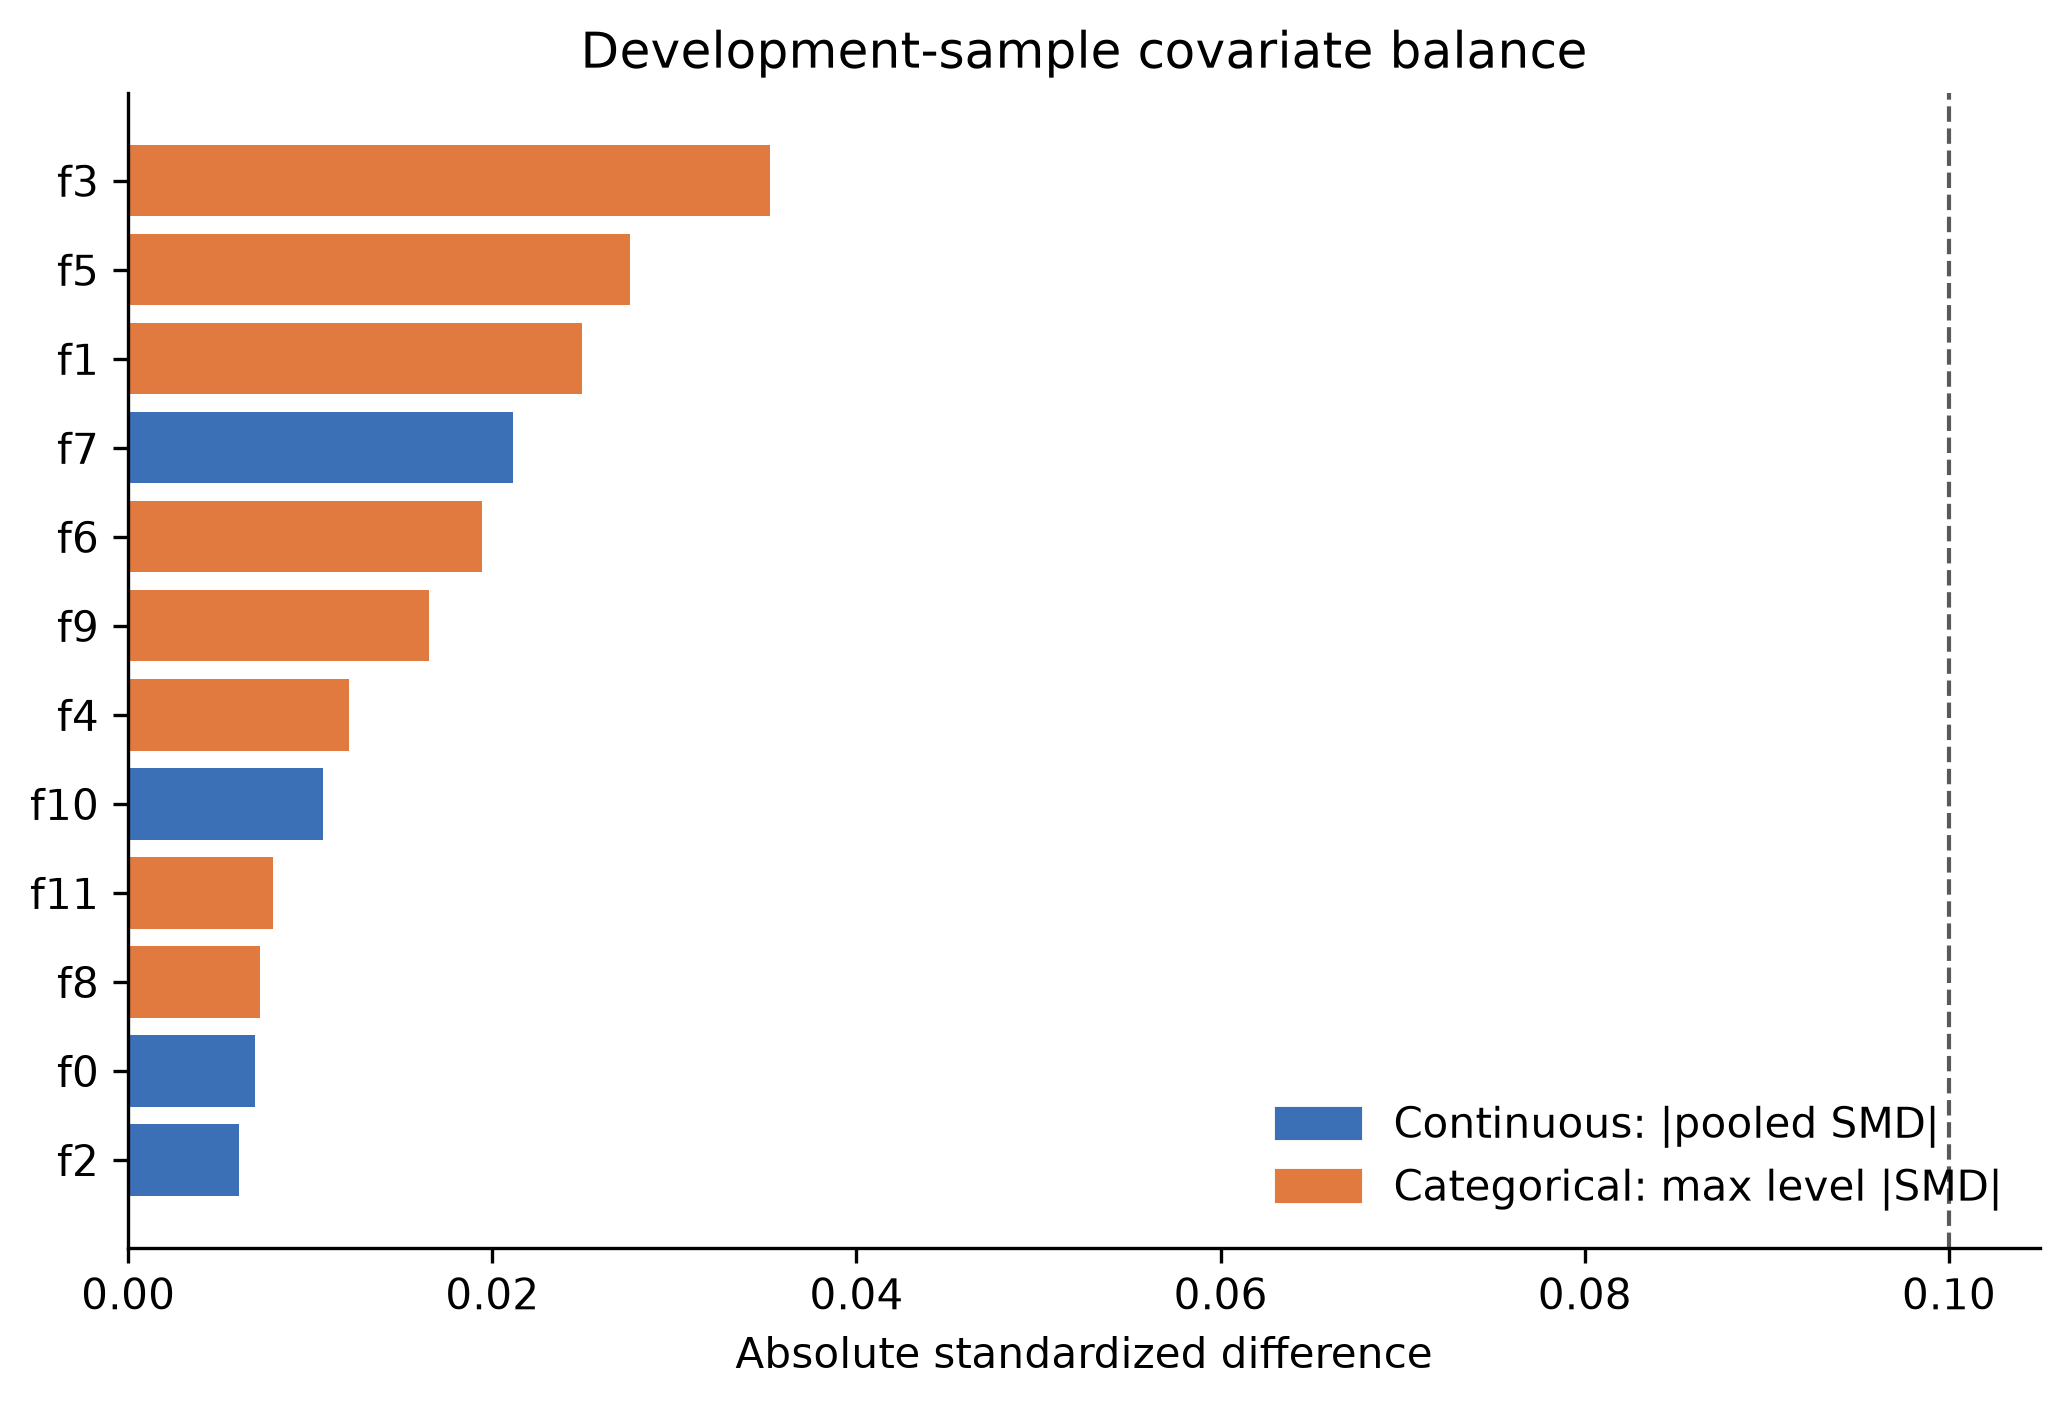
\includegraphics[width=0.84\textwidth]{figures/balance.png}
\caption{Training-and-validation covariate balance. Continuous features use pooled SMDs; categorical features use the largest absolute one-versus-rest SMD across levels. The 0.1 reference line is descriptive.}
\label{fig:balance}
\end{figure}

The complete-source conversion ATE was 0.1152 percentage points (95\% confidence interval 0.1085 to 0.1219). The visit ATE was 1.0342 percentage points (1.0056 to 1.0629). Table~\ref{tab:ate} reports analytic standard errors and group sizes.

\begin{table}[htbp]
\centering
\caption{Complete-source difference-in-means average treatment effects. Units are percentage points (pp).}
\label{tab:ate}
\resizebox{\textwidth}{!}{\begin{tabular}{@{}lrrrr@{}}
\toprule
Outcome & Estimate (pp) & SE (pp) & 95\% CI (pp) & Treated / control $n$ \\
\midrule
Conversion & 0.1152 & 0.0034 & [0.1085, 0.1219] & 11,882,655 / 2,096,937 \\
Visit & 1.0342 & 0.0146 & [1.0056, 1.0629] & 11,882,655 / 2,096,937 \\
\bottomrule
\end{tabular}
}
\end{table}

\subsection{Held-out conversion policy value}

Figure~\ref{fig:policy-values} shows the primary and secondary policy value estimates. For conversion, the treated-response score had the highest point estimate at 5\%, 10\%, 20\%, and 50\% capacity. At 10\%, the estimated values per 100,000 eligible test users were 9.8 for random allocation, 87.1 for treated-response, 78.1 for the T-learner, and 57.4 for the DR-learner (Table~\ref{tab:conversion-values}).

\begin{figure}[htbp]
\centering
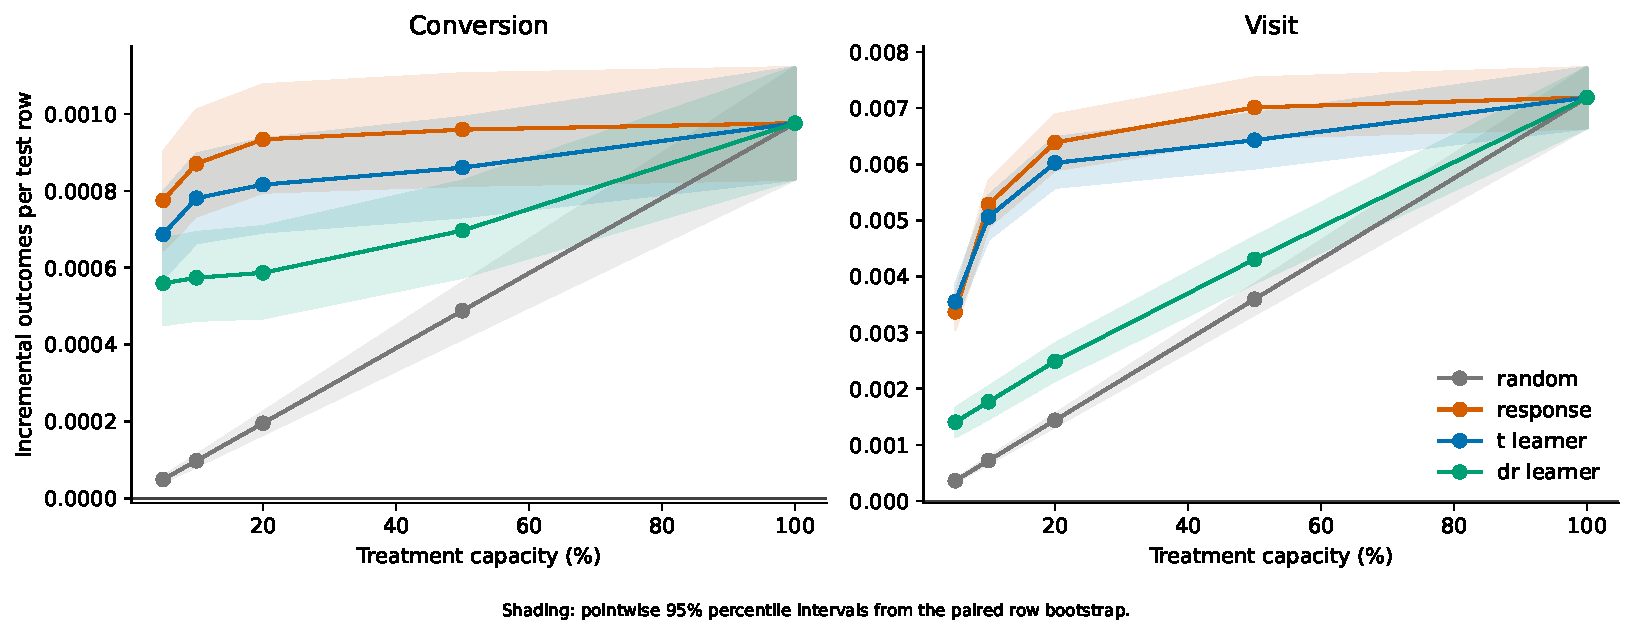
\includegraphics[width=\textwidth]{figures/policy_values.pdf}
\caption{Held-out AIPW policy value by treatment capacity. Policies are ranked by conversion scores; the right panel evaluates visit for those same policies. Shading gives pointwise 95\% percentile intervals from the paired row bootstrap, conditional on fitted models.}
\label{fig:policy-values}
\end{figure}

\begin{table}[htbp]
\centering
\caption{Held-out conversion policy value per 100,000 eligible test users. Cells report estimate [pointwise 95\% percentile interval].}
\label{tab:conversion-values}
\resizebox{\textwidth}{!}{\begin{tabular}{@{}rllll@{}}
\toprule
Capacity (\%) & Random & Treated-response & T-learner & DR-learner \\
\midrule
5 & 4.9 [4.2, 5.6] & 77.5 [64.7, 90.1] & 68.7 [57.2, 79.6] & 56.0 [45.1, 67.5] \\
10 & 9.8 [8.3, 11.2] & 87.1 [73.5, 101.0] & 78.1 [66.5, 89.6] & 57.4 [46.3, 69.2] \\
20 & 19.5 [16.6, 22.4] & 93.4 [79.6, 107.6] & 81.6 [69.3, 93.5] & 58.7 [46.9, 70.7] \\
50 & 48.8 [41.5, 56.0] & 95.9 [81.4, 110.5] & 86.0 [73.2, 99.1] & 69.7 [57.5, 82.5] \\
100 & 97.6 [83.0, 112.1] & 97.6 [83.0, 112.1] & 97.6 [83.0, 112.1] & 97.6 [83.0, 112.1] \\
\bottomrule
\end{tabular}
}
\end{table}

Paired contrasts sharpen the comparison because every policy is evaluated on the same resampled test rows. At 10\% capacity, treated-response exceeded expected random allocation by 77.3 incremental conversions per 100,000 (pointwise 95\% interval 65.1 to 90.0). It exceeded the T-learner by 9.0 (1.8 to 15.3) and the DR-learner by 29.7 (21.8 to 37.5). For each of the four constrained capacities, each of these pre-specified pointwise intervals excluded zero in the treated-response direction. This statement is pointwise and is not adjusted for testing across capacities.

\begin{figure}[htbp]
\centering
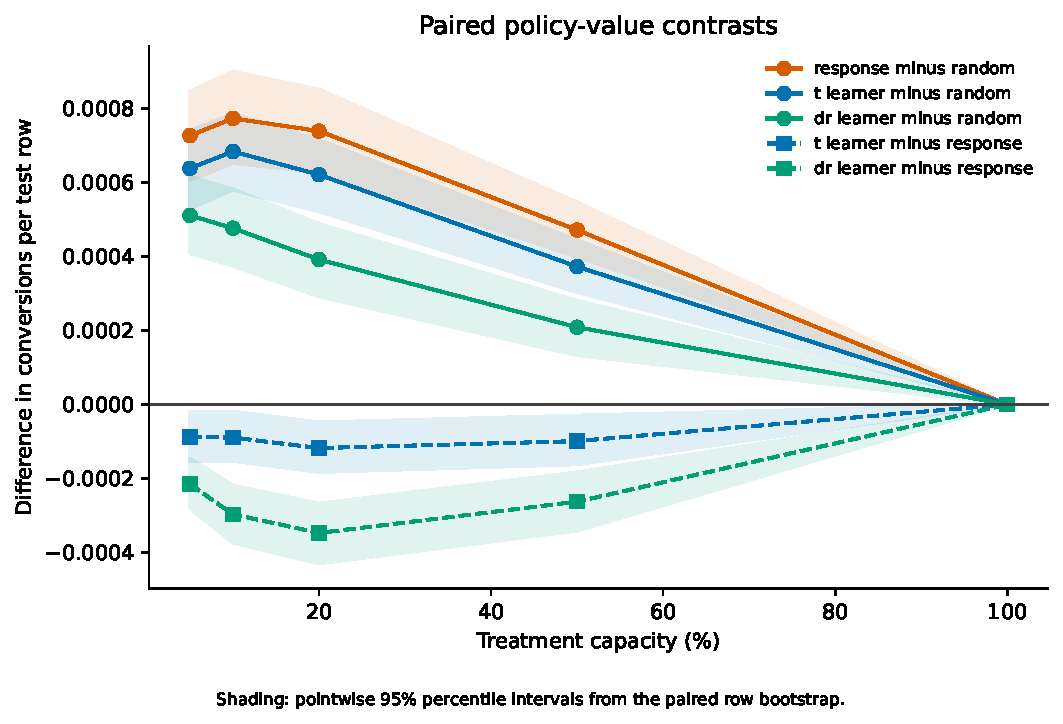
\includegraphics[width=0.82\textwidth]{figures/conversion_policy_contrasts.pdf}
\caption{Paired held-out conversion policy-value contrasts. Solid circles compare fitted policies with expected exact-size random allocation. Dashed squares compare the T-learner and DR-learner with treated-response. Shading gives pointwise 95\% percentile intervals from the paired row bootstrap, conditional on fitted models.}
\label{fig:conversion-contrasts}
\end{figure}

\begin{table}[htbp]
\centering
\caption{Paired conversion policy-value contrasts per 100,000 eligible test users. Cells report estimate [pointwise 95\% percentile interval].}
\label{tab:conversion-contrasts}
\resizebox{\textwidth}{!}{\begin{tabular}{@{}rlll@{}}
\toprule
Capacity (\%) & Response $-$ random & Response $-$ T-learner & Response $-$ DR-learner \\
\midrule
5 & 72.6 [60.5, 84.7] & 8.8 [1.8, 15.4] & 21.5 [14.5, 28.1] \\
10 & 77.3 [65.1, 90.0] & 9.0 [1.8, 15.3] & 29.7 [21.8, 37.5] \\
20 & 73.9 [62.7, 85.2] & 11.8 [4.7, 18.4] & 34.7 [26.7, 43.1] \\
50 & 47.1 [39.9, 54.7] & 9.9 [2.9, 16.3] & 26.3 [18.2, 34.2] \\
100 & 0.0 [0.0, 0.0] & 0.0 [0.0, 0.0] & 0.0 [0.0, 0.0] \\
\bottomrule
\end{tabular}
}
\end{table}

At 100\% capacity, all four values equal 97.6 incremental conversions per 100,000. The corresponding contrasts are exactly zero because every rule treats the entire test set. This equality follows from the policy definition; it does not imply that the rankings are equivalent.

\subsection{Qini ranking diagnostic}

The centered fixed-propensity IPW Qini curves give the same ordering of the three fitted scores (Figure~\ref{fig:qini}). The treated-response coefficient was $5.127\times10^{-4}$ per test row, compared with $3.651\times10^{-4}$ for the T-learner and $2.258\times10^{-4}$ for the DR-learner. The Qini calculation uses transformed outcomes rather than AIPW scores, so numerical agreement with policy values is neither expected nor required.

\begin{figure}[htbp]
\centering
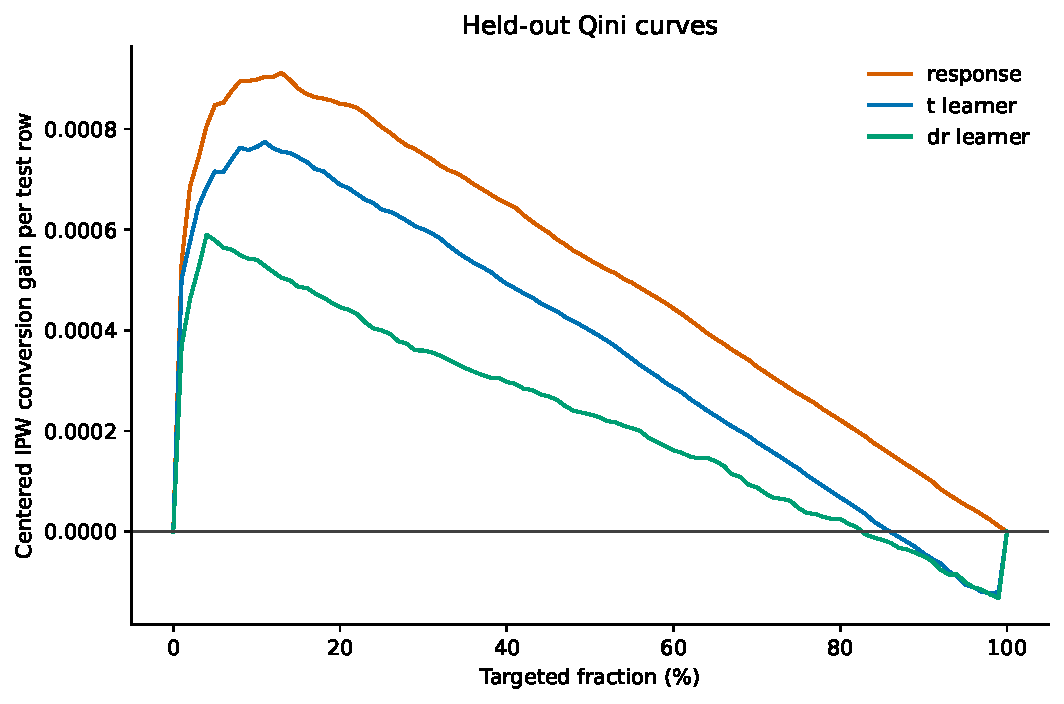
\includegraphics[width=0.82\textwidth]{figures/qini_curves.pdf}
\caption{Centered fixed-propensity IPW Qini curves for conversion. The displayed curves use 101 points; coefficients use the full test ordering.}
\label{fig:qini}
\end{figure}

\begin{table}[htbp]
\centering
\caption{Full-resolution centered Qini coefficients on the held-out test set.}
\label{tab:qini}
\begin{tabular}{@{}lr@{}}
\toprule
Ranking score & Qini coefficient ($\times 10^{4}$) \\
\midrule
Treated-response & 5.127 \\
T-learner & 3.651 \\
DR-learner & 2.258 \\
\bottomrule
\end{tabular}

\end{table}

\subsection{Secondary visit outcome}

All three fitted conversion policies had higher estimated visit value than random allocation at each constrained capacity. Comparisons between treated-response and the T-learner were less uniform than for conversion. At 5\%, the T-learner's point estimate was 18.1 visits per 100,000 above treated-response, with a pointwise interval from $-0.02$ to 37.1. At 10\%, treated-response was 22.0 above the T-learner, with an interval from $-1.6$ to 46.3. Both intervals included zero. Treated-response was higher at 20\% and 50\%, with pointwise intervals that excluded zero. It exceeded the DR-learner across all constrained capacities. These are secondary comparisons of policies trained to rank conversion, not separately optimized visit policies.

\subsection{Estimator and sample boundaries}

Table~\ref{tab:estimator-scope} prevents three valid but different estimates from being conflated. The complete-source difference-in-means ATE is 115.2 incremental conversions per 100,000. The raw difference in test assignment-group means is 111.0. The held-out AIPW value of treating every test row is 97.6, with a pointwise interval that contains the raw test difference. The values differ because they use different samples and, for the last row, regression adjustment. The full-capacity AIPW estimate is not intended to reproduce the complete-source difference in means.

\begin{table}[htbp]
\centering
\caption{Conversion quantities with different samples or estimators. Bracketed values are 95\% intervals.}
\label{tab:estimator-scope}
\resizebox{\textwidth}{!}{\begin{tabular}{@{}lll@{}}
\toprule
Quantity & Sample and estimator & Incremental conversions per 100,000 \\
\midrule
Average treatment effect & Complete source, difference in means & 115.2 [108.5, 121.9] \\
Raw assignment difference & Held-out test, difference in means & 111.0 (no interval reported) \\
All-treatment policy value & Held-out test, AIPW & 97.6 [83.0, 112.1] \\
\bottomrule
\end{tabular}
}
\end{table}

\FloatBarrier

\section{Discussion}

The main empirical finding is narrow: among the four frozen rules, treated-response ranking produced the highest held-out estimated conversion policy value whenever capacity was constrained. The paired contrast intervals exclude zero at the four pre-specified constrained capacities. Among these four rules, this evidence favors treated-response for the present benchmark and model specification; it does not establish that response ranking is generally optimal.

The result is compatible with the causal bias-variance tradeoff analyzed by \citet{fernandezloria2022causal}. A treated-response score can be biased for an individual treatment effect but still order decisions well when estimating a difference between two rare-outcome response surfaces adds enough variance. The present analysis does not identify why the response score won. It did not measure CATE ground truth, decompose ranking error, or vary model classes and training sizes. Rare conversion, arm imbalance, response-effect association, and learner specification are possible explanations, not tested mechanisms.

The DR-learner's lower ranking value does not contradict doubly robust theory. Theoretical robustness concerns nuisance estimation and target estimation under stated conditions \citep{chernozhukov2018dml,kennedy2023dr}; it does not guarantee that every fitted DR regression will yield the best finite-sample top-$k$ ordering. Here the second-stage regressor selected ten boosting rounds by a fixed validation rule, and that procedure was not revisited after test outcomes were observed.

Qini and policy value answered related but distinct questions. The centered IPW Qini coefficient summarized the full ordering, whereas the AIPW analysis evaluated exact allocations at five capacities. Their ordering agreed in this experiment. That agreement should not be assumed in another dataset because the metrics weight ranks differently and use different scores for outcome adjustment.

The capacity formulation also limits the business interpretation. Each selected user consumes one abstract slot. Without treatment cost, conversion value, or heterogeneous resource use, no monetary optimization is identified. An analyst could apply external values and costs to these estimates as a scenario calculation, but such a calculation would not become a measured return from the Criteo data.

\section{Limitations}

The evidence comes from one anonymized advertising benchmark. Feature semantics, advertiser identifiers, time order, and deployment context are unavailable. The hash split treats rows as IID. It cannot account for advertiser clusters, repeated users, campaign dependence, or temporal shifts. The released-data population may also differ from live traffic because the publisher anonymized and sampled the original experiments.

Inference is conditional on the fitted models. The paired row bootstrap recomputes cutoffs and policy contrasts, but it does not refit nuisance or ranking models. The reported intervals are pointwise, with no family-wise adjustment across capacities or policies. Model-selection uncertainty, simultaneous bands, and uncertainty under clustered sampling remain outside scope.

The study compares a deliberately small policy set with one fixed LightGBM specification. It does not establish an oracle ranking or survey every uplift method. Treatment is randomized assignment and exposure is post-assignment, so excluding exposure gives an intention-to-treat analysis. The results do not estimate effects among exposed users. Finally, exact top-$k$ batch allocation presumes that all candidate scores are available together. Online arrival, delayed outcomes, treatment fatigue, and changing inventory would require another policy design and prospective validation.

\section{Conclusion}

On the corrected CRITEO-UPLIFTv2 release, treated-response ranking had higher held-out estimated conversion policy value than random, T-learner, and DR-learner rankings at capacities of 5\%, 10\%, 20\%, and 50\%. Each pre-specified pointwise paired interval favored treated-response at these capacities. At full capacity, all policies were identical by construction, and the separately defined Qini diagnostic gave the same ordering of fitted scores.

Policy scores therefore need direct evaluation under the decision rule and capacity of interest; predictive or CATE-oriented metrics alone do not establish policy value. In this benchmark, estimating treatment effects explicitly did not guarantee the best finite-sample allocation among the tested methods. Claims beyond the released distribution require richer cost data, deployment structure, and prospective evaluation.

\section*{Reproducibility and data availability}

Code, configuration, aggregate results, manuscript source, and provenance manifests are available in the
\href{https://github.com/felixxaxs12/budget-constrained-uplift-modelling-and-causal-policy-optimization}{public project repository}.
The repository records the exact software versions, selected boosting rounds, data digest, and model hashes used for the reported run. Generated manuscript tables read the canonical aggregate CSV files; they do not duplicate statistical calculations.

The raw Criteo dataset is not redistributed. The repository downloads the corrected artifact from the publisher and verifies its byte size, gzip integrity, ordered schema, row count, and SHA-256 digest. The dataset is licensed separately under CC BY-NC-SA 4.0 \citep{criteoDataset}. Project code is licensed under MIT, and the manuscript is licensed under CC BY 4.0.

\section*{Ethics statement}

This study is a secondary analysis of a public, anonymized benchmark. It collected no new participant data and assigned no new intervention. The analysis retains the publisher's anonymous feature names and reports only aggregate results. Treatment is analyzed as randomized assignment; the post-assignment exposure field is excluded from modelling.

\section*{AI assistance disclosure}

OpenAI Codex assisted with literature retrieval, code implementation, execution orchestration, language editing, and manuscript review. The cited sources were checked against primary or publisher records, and reported results were verified against committed aggregate artifacts. No generative output was used as research data. OpenAI Codex is not an author; responsibility for any submitted version rests with Yi Zhao.

\appendix

\section{Implementation details}

Table~\ref{tab:model-selection} reports the frozen boosting rounds and validation losses. Binary models use log-loss. For DR round selection, the regressor is fitted on three-fold out-of-fold training pseudo-outcomes and evaluated by mean squared error against validation pseudo-outcomes formed with train-fitted nuisance models. The final DR regressor is then fitted on three-fold out-of-fold pseudo-outcomes from the combined development sample. The fitted artifacts were produced with Python 3.13.1, LightGBM 4.7.0, NumPy 2.5.1, and pandas 3.0.5.

\begin{table}[htbp]
\centering
\caption{Model selection recorded before held-out outcome evaluation.}
\label{tab:model-selection}
\begin{tabular}{@{}lrr@{}}
\toprule
Model & Selected rounds & Validation loss \\
\midrule
Conversion $\widehat m_0$ & 59 & 0.008349 \\
Conversion $\widehat m_1$ & 95 & 0.012734 \\
Visit $\widehat m_0$ & 121 & 0.090270 \\
Visit $\widehat m_1$ & 236 & 0.105710 \\
DR-learner & 10 & 0.014024 \\
\bottomrule
\end{tabular}

\end{table}

The fitted-model freeze manifest has SHA-256 digest
\texttt{\small 140113d9dcb4bfe6bc0b4968414b5393\allowbreak 556d2f29c18a4bd8addfe9c9da5ed30a}.
The evaluation manifest records a clean source commit, verifies the tracked freeze manifest, and confirms that predictions were created before test outcome columns were loaded for evaluation.

\section{Secondary visit contrasts}

Table~\ref{tab:visit-contrasts} gives the complete secondary contrast results. The directions are written as treated-response minus comparator for readability; the underlying paired estimates are preserved by sign reversal where needed.

\begin{table}[htbp]
\centering
\caption{Paired visit policy-value contrasts per 100,000 eligible test users. Cells report estimate [pointwise 95\% percentile interval]. Policies are ranked by conversion scores.}
\label{tab:visit-contrasts}
\resizebox{\textwidth}{!}{\begin{tabular}{@{}rlll@{}}
\toprule
Capacity (\%) & Response $-$ random & Response $-$ T-learner & Response $-$ DR-learner \\
\midrule
5 & 300.9 [271.8, 330.2] & -18.1 [-37.1, 0.0] & 196.4 [175.4, 216.7] \\
10 & 456.3 [421.7, 493.7] & 22.0 [-1.6, 46.3] & 351.5 [319.0, 384.7] \\
20 & 495.1 [456.3, 535.3] & 36.5 [12.0, 62.6] & 390.0 [350.8, 434.7] \\
50 & 341.6 [313.8, 368.2] & 58.2 [34.0, 81.3] & 270.5 [234.6, 306.2] \\
100 & 0.0 [0.0, 0.0] & 0.0 [0.0, 0.0] & 0.0 [0.0, 0.0] \\
\bottomrule
\end{tabular}
}
\end{table}

\bibliographystyle{plainnat}
\bibliography{references}

\end{document}
